%!TEX root =  main.tex

\lectureheader{162}{Calculus II}{Hyperbolic functions}{\textit{Thomas' Calculus}  7.7}

\begin{definition}
We define the \textbf{hyperbolic sine} by the rule
\begin{equation*}
\sinh x = \frac{\E^x-\E^{-x}}{2} \quad (x\in\R)
\end{equation*}
and the \textbf{hyperbolic cosine} by the rule
\begin{equation*}
\cosh x = \frac{\E^x+\E^{-x}}{2} \quad (x\in\R).
\end{equation*}
\end{definition}

\begin{remark}\,
\begin{itemize}
\item These functions are affectionately referred to as ``cinch" and ``kosh."
\item The ordinary sine and cosine are sometimes called ``circular" functions because they parameterize circles.
If $t\in [0,2\pi)$, then the point $(x,y) = (\cos t, \sin t)$ lies on the circle
\begin{equation*}
x^2+y^2=1.
\end{equation*}
\item These hyperbolic analogues parameterize hyperbolas.
If $t\in (-\infty,\infty)$, then the point $(x,y)=(\cosh t, \sinh t)$ lies on the right branch of the hyperbola
\begin{equation*}
x^2-y^2=1.
\end{equation*}
\end{itemize}
\end{remark}

\begin{definition}
We define the \textbf{hyperbolic tangent} by the rule
\begin{equation*}
\tanh x = \frac{\sinh x}{\cosh x} \quad (x\in \R),
\end{equation*}
the \textbf{hyperbolic cosecant} by the rule
\begin{equation*}
\csch x = \frac{1}{\sinh x} \quad (x\ne 0),
\end{equation*}
the \textbf{hyperbolic secant} by the rule
\begin{equation*}
\sech x = \frac{1}{\cosh x} \quad (x\in\R),
\end{equation*}
and the \textbf{hyperbolic cotangent} by the rule
\begin{equation*}
\coth x = \frac{\cosh x}{\sinh x} \quad (x\ne 0).
\end{equation*}
\end{definition}

\newpage

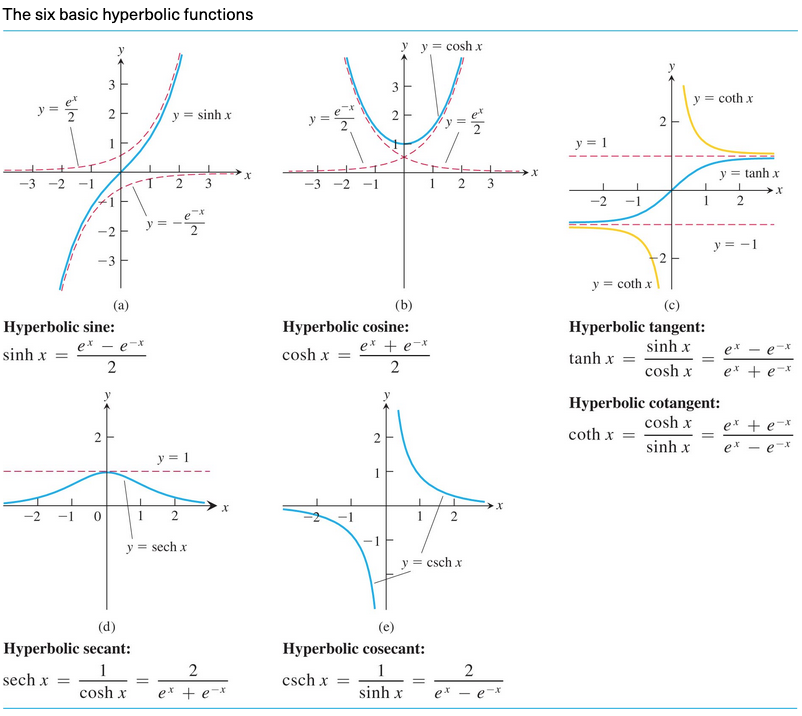
\includegraphics[width=6.5in]{img/hyperbolic_graphs}

\newpage

\begin{theorem}
For all $x$ where both sides of the identity are defined we have 
\begin{align}
\cosh^2 x -\sinh^2 x &= 1, \label{hyperbolic trig identity}\\ 
1-\tanh^2x &=\sech^2 x,\\
\coth^2 x -1&=\csch^2 x,\\
\sinh 2x &= 2\sinh x\cosh x,\\
\cosh 2x &=\cosh^2x + \sinh^2 x,\\
\cosh^2 x&=\frac{\cosh 2x + 1}{2},\\
\sinh^2 x&=\frac{\cosh 2x - 1}{2}.
\end{align}
\end{theorem}
\ifdefined\SOLUTION
\SOLUTION[Proof of \eqref{hyperbolic trig identity}] {
For all $x\in (-\infty, \infty)$,
\begin{align*}
    \cosh^2{x} - \sinh^2{x} &= \left(\frac{\E^x+\E^{-x}}{2}\right)^2 - \left(\frac{\E^x-\E^{-x}}{2}\right)^2 \\
    &= \frac{\E^{2x} + 1 + 1 + \E^{-2x}}{4} - \frac{\E^{2x} + 1 + 1 + \E^{-2x}}{4} \\
    &= \frac{(\E^{2x} + 1 + 1 + \E^{-2x}) - (\E^{2x} + 1 + 1 + \E^{-2x})}{4} \\
    &= \frac{4}{4} \\
    &= 1. \\
\end{align*}
}
\else
\begin{proof}[Proof of \eqref{hyperbolic trig identity}]\,

\vspace{5in}
\end{proof}
\fi
\newpage

\begin{theorem}
\begin{align}
\frac{\dee}{\dee x}\sinh x &= \cosh x\quad (x\in\R)\label{sinh derivative}\\
\frac{\dee}{\dee x}\cosh x &= \sinh x\quad (x\in\R)\\
\frac{\dee}{\dee x}\tanh x &= \sech^2 x\quad (x\in\R) \label{sech derivative}\\
\frac{\dee}{\dee x}\csch x &= -\csch x\coth x\quad (x\ne 0)\\
\frac{\dee}{\dee x}\sech x &= -\sech x\tanh x\quad (x\in \R)\\
\frac{\dee}{\dee x}\coth x &= -\csch^2 x\quad (x\ne 0)
\end{align}
\end{theorem}
\begin{remark}
Of course, each of these gives rise to a corresponding integral formula.
\end{remark}
\ifdefined\SOLUTION
\SOLUTION[Proof of \eqref{sech derivative}]{
For $x\in (-\infty, \infty)$,
\begin{align*}
\frac{\dee}{\dee x}\sech{x} 
	&= \frac{\dee}{\dee x} (\cosh{x})^{-1}\\
    &= -(\cosh{x})^{-2}\cdot\frac{\dee}{\dee x}\cosh{x} \\
    &= -(\cosh{x})^{-2}\sinh{x}\\ %\quad \text{(by~\eqref{sinh derivative})} \\
    &=-\tanh(x)\sech(x). 
\end{align*}
}
\else
\begin{proof}[Proof of \eqref{sech derivative}]\,

\vspace{5in}
\end{proof}
\fi

\newpage

\begin{example}
Compute $\dee y/\dee x$ if $y=\tanh \sqrt{1+x^2}$.
\end{example}
\ifdefined\SOLUTION
\SOLUTION[Solution]{
\begin{align*}
    \frac{\dee y}{\dee x} &= \left(\sech^2{\sqrt{1+x^2}}\right)\cdot\frac{\dee}{\dee x}(1+x^2)^\frac{1}{2} \\
    &= \left(\sech^2{\sqrt{1+x^2}}\right)\cdot\frac{1}{2}(1+x^2)^{-1/2}\cdot\frac{\dee}{\dee x}(1+x^2) \\
    &=  \frac{\left(\sech^2{\sqrt{1+x^2}}\right)}{2\sqrt{1+x^2}}\cdot 2x \\
    &= \frac{x\sech^2{\sqrt{1+x^2}}}{\sqrt{1+x^2}}. 
\end{align*}
}
\else
\fi
\vfill

\begin{example}
Compute $\DS\int\sinh^2 x\dee x$
\end{example}
\ifdefined\SOLUTION
\SOLUTION[Solution]{
One way to evaluate this integral is 
\begin{align*}
    \int\sinh^2 x\dee x &= \int\left(\frac{\E^x+\E^{-x}}{2}\right)^2\dee x \\
    &= \frac{1}{4}\int(\E^{2x} - 2 + \E^{-2x})\dee x \\
    &= \frac{1}{4}\left[ \frac{1}{2}\E^{2x} - 2x - \frac{1}{2}\E^{-2x} \right] + C \\
    &= \frac{1}{4}\left[ \sinh{2x} - 2x \right] + C.
\end{align*}
Another way to evaluate this integral is 
\begin{align*}
    \int\sinh^2 x\dee x &= \int\frac{\cosh{(2x} - 1)}{2}\dee x \\
    &= \frac{1}{2} \left[ \frac{1}{2}\sinh{(2x)} - x \right] + C \\
    &= \frac{1}{4}\sinh{(2x)} - \frac{1}{2}x + C.
\end{align*}
}
\else
\fi
\vfill

\newpage

\begin{example}
What is the domain/range of $y=\sinh x$?
Where can we invert it?
\end{example}
\ifdefined\SOLUTION
\SOLUTION[Solution]{
Since $\sinh(x) = \frac{\E^x-\E^{-x}}{2}$, we see that $\dom(\sinh) = (-\infty, \infty)$ and $\rng(\sinh) = (-\infty, \infty)$.  
Now note that
\begin{equation*}
    \frac{\dee}{\dee x}\sinh{x} = \cosh{x} = \frac{\E^x+\E^{-x}}{2} > 0
\end{equation*}
for all $x\in (-\infty, \infty)$.
Therefore, $\sinh{x}$ is 1-1 and thus invertible everywhere.  So, $\arcsinh{x} = \sinh^{-1}{x}$ exists and $\dom(\arcsinh) = (-\infty, \infty)$ and $\rng(\arcsinh) = (-\infty, \infty)$.
}
\else
\fi
\vfill

\begin{example}
What is the domain/range of $y=\cosh x$?
Where can we invert it?
\end{example}
\ifdefined\SOLUTION
\SOLUTION[Solution]{
Since $\cosh(x) = \frac{\E^x+\E^{-x}}{2}$, we see that $\dom(\cosh) = (-\infty,\infty)$ and $\rng(\cosh) = [1, \infty)$.
Now note that
\begin{equation*}
    \frac{\dee}{\dee x}\cosh{x} = \sinh{x} = \frac{\E^x-\E^{-x}}{2} > 0 
\end{equation*}
for all $x\in [0,\infty)$.
So, we can invert the right half of cosh, i.e., $\cosh^{-1}{x}$ exists, but $\dom(\cosh^{-1}) = [1, \infty)$ and $\rng(\cosh^{-1}) = [0, \infty).$
}
\else
\fi
\vfill

\newpage

\begin{definition}
The six ``inverse" hyperbolic functions are defined by the rules:
\begin{enumerate}
\item $y=\sinh^{-1} x\quad (x\in\R) \iff \sinh y = x\quad (y\in\R)$.
\item $y = \cosh^{-1} x\quad (x\ge 1) \iff \cosh y = x\quad (0\le y<\infty)$.
\item $y = \tanh^{-1} x\quad (|x|<1) \iff \tanh y = x\quad (y\in\R)$ 
\item $y=\csch^{-1} x\quad (x\ne 0)\iff \csch y = x\quad (y\ne 0)$.
\item $y = \sech^{-1} x\quad (0<x\le 1) \iff \sech y = x\quad (y\ge 0)$.
\item $y = \coth^{-1} x\quad (|x|>1) \iff \coth y = x\quad (y\ne 0)$.
\end{enumerate}
\end{definition}
\begin{remark}\,
\begin{itemize}
\item Four of these are ``true" inverses while the other two are only ``partial" inverses.
Can you figure out which?
\item We also use the notation $\arcsinh x = \sinh^{-1} x$, etc.
\end{itemize}
\end{remark}

\begin{theorem}
\begin{align}
\frac{\dee}{\dee x}\sinh^{-1} x & = \frac{1}{\sqrt{1+x^2}}\label{inverse sinh derivative}\\
\frac{\dee}{\dee x}\cosh^{-1} x & = \frac{1}{\sqrt{x^2-1}}\quad (x>1)\\
\frac{\dee}{\dee x}\tanh^{-1} x & = \frac{1}{1-x^2}\quad (|x|<1)\\
\frac{\dee}{\dee x}\csch^{-1} x &=\frac{-1}{|x|\sqrt{1+x^2}}\quad (x\ne 0) \label{inverse csch derivative} \\
\frac{\dee}{\dee x}\sech^{-1} x & = \frac{-1}{x\sqrt{1-x^2}}\quad (0<x<1)\\
\frac{\dee}{\dee x}\coth^{-1} x & = \frac{1}{1-x^2}\quad (|x|>1)
\end{align}
\end{theorem}
\ifdefined\SOLUTION
\SOLUTION[Proof of \eqref{inverse sinh derivative}]{
First observe that
\begin{equation*}
\sinh(\sinh^{-1}(x)) = x \quad (x\in\R).  
\end{equation*}
Differentiating both sides, we find that
\begin{equation*}
\cosh(\sinh^{-1} x)\frac{\dee}{\dee x}\sinh^{-1} x = 1.
\end{equation*}
Dividing, we have
\begin{equation*}
\frac{\dee}{\dee x}\sinh^{-1} x = \frac{1}{\cosh(\sinh^{-1} x)}.
\end{equation*}
Since $\cosh(z)>0$ for all $z\in\R$, it follows that
\begin{equation*}
\cosh(\sinh^{-1} x) = |\cosh(\sinh^{-1} x)|
 = \sqrt{\cosh^2(\sinh^{-1} x)}
 = \sqrt{1+\sinh^2(\sinh^{-1} x)}
 = \sqrt{1+x^2}.
\end{equation*}
Therefore,
\begin{equation*}
\frac{\dee}{\dee x}\sinh^{-1} x = \frac{1}{\sqrt{1+x^2}}.
\end{equation*}
}
\else
\begin{proof}[Proof of \eqref{inverse sinh derivative}]\,

\vspace{2.75in}
\end{proof}
\fi

\newpage

\begin{theorem}
\begin{align}
\int\frac{\dee x}{\sqrt{1+x^2}} &= \sinh^{-1} x + C;\\
\int\frac{\dee x}{\sqrt{x^2-1}} & = \cosh^{-1} x + C\quad (x>1);\\
\int\frac{\dee x}{1-x^2} 
&=\begin{cases}
\tanh^{-1} x + C& \text{if } |x|<1,\\
\coth^{-1} x + C& \text{if } |x|>1;
\end{cases}\\
\int\frac{\dee x}{x\sqrt{1-x^2}} &= -\sech^{-1} x + C\quad (0<x<1);\\
\int\frac{\dee x}{x\sqrt{1+x^2}} &=-\csch^{-1} |x| + C\quad (x\ne 0).
\end{align}
\end{theorem}

\begin{example}
Evaluate $\DS\int_0^1\frac{2\dee x}{\sqrt{3+4x^2}}$.
\end{example}
\ifdefined\SOLUTION
\SOLUTION[Solution]{
First note that
\begin{equation*}
    \int_0^1\frac{2\dee x}{\sqrt{3+4x^2}}
    = \int_0^1\frac{2\dee x}{\sqrt{3}\sqrt{1 + \left( \frac{2x}{\sqrt{3}} \right)^2}}.
\end{equation*}
Now let $u = \frac{2x}{\sqrt 3}$ so that $\dee u = \frac{2}{\sqrt 3}\dee x$.  
Furthermore, if $x = 0$, then $u = 0$, and if $x = 1$, then $u = \frac{2}{\sqrt{3}}$.
Making the substitution gives
\begin{equation*}
    \int_0^{\frac{2}{\sqrt{3}}} \frac{\dee u}{\sqrt{1+u^2}}
    = \arcsinh{\frac{2}{\sqrt 3}} - \arcsinh{0}
    = \arcsinh{\frac{2}{\sqrt 3}}.
\end{equation*}
}
\else
\fi
